% GNUPLOT: LaTeX picture with Postscript
\documentclass{minimal}
% Set font size
\makeatletter
\def\@ptsize{1}
\InputIfFileExists{size11.clo}{}{%
   \GenericError{(gnuplot) \space\space\space\@spaces}{%
      Gnuplot Error: File `size11.clo' not found! Could not set font size%
   }{See the gnuplot documentation for explanation.%
   }{For using a font size a file `size<fontsize>.clo' has to exist.
        Falling back ^^Jto default fontsize 10pt.}%
  \def\@ptsize{0}
  \input{size10.clo}%
}%
\makeatother
% Load packages
\usepackage{calc}
\usepackage{graphicx}
\usepackage{color}
\makeatletter
% Select an appropriate default driver (from TeXLive graphics.cfg)
\begingroup
  \chardef\x=0 %
  % check pdfTeX
  \@ifundefined{pdfoutput}{}{%
    \ifcase\pdfoutput
    \else
      \chardef\x=1 %
    \fi
  }%
  % check VTeX
  \@ifundefined{OpMode}{}{%
    \chardef\x=2 %
  }%
\expandafter\endgroup
\ifcase\x
  % default case
  \PassOptionsToPackage{dvips}{geometry}
\or
  % pdfTeX is running in pdf mode
  \PassOptionsToPackage{pdftex}{geometry}
\else
  % VTeX is running
  \PassOptionsToPackage{vtex}{geometry}
\fi
\makeatother
% Set papersize
\usepackage[papersize={360.00bp,252.00bp},text={360.00bp,252.00bp}]{geometry}
% No page numbers and no paragraph indentation
\pagestyle{empty}
\setlength{\parindent}{0bp}%
% Load configuration file
\InputIfFileExists{gnuplot.cfg}{%
  \typeout{Using configuration file gnuplot.cfg}%
}{%
 \typeout{No configuration file gnuplot.cfg found.}%
}%
%
\begin{document}
\begingroup
  \makeatletter
  \providecommand\color[2][]{%
    \GenericError{(gnuplot) \space\space\space\@spaces}{%
      Package color not loaded in conjunction with
      terminal option `colourtext'%
    }{See the gnuplot documentation for explanation.%
    }{Either use 'blacktext' in gnuplot or load the package
      color.sty in LaTeX.}%
    \renewcommand\color[2][]{}%
  }%
  \providecommand\includegraphics[2][]{%
    \GenericError{(gnuplot) \space\space\space\@spaces}{%
      Package graphicx or graphics not loaded%
    }{See the gnuplot documentation for explanation.%
    }{The gnuplot epslatex terminal needs graphicx.sty or graphics.sty.}%
    \renewcommand\includegraphics[2][]{}%
  }%
  \providecommand\rotatebox[2]{#2}%
  \@ifundefined{ifGPcolor}{%
    \newif\ifGPcolor
    \GPcolorfalse
  }{}%
  \@ifundefined{ifGPblacktext}{%
    \newif\ifGPblacktext
    \GPblacktexttrue
  }{}%
  % define a \g@addto@macro without @ in the name:
  \let\gplgaddtomacro\g@addto@macro
  % define empty templates for all commands taking text:
  \gdef\gplbacktext{}%
  \gdef\gplfronttext{}%
  \makeatother
  \ifGPblacktext
    % no textcolor at all
    \def\colorrgb#1{}%
    \def\colorgray#1{}%
  \else
    % gray or color?
    \ifGPcolor
      \def\colorrgb#1{\color[rgb]{#1}}%
      \def\colorgray#1{\color[gray]{#1}}%
      \expandafter\def\csname LTw\endcsname{\color{white}}%
      \expandafter\def\csname LTb\endcsname{\color{black}}%
      \expandafter\def\csname LTa\endcsname{\color{black}}%
      \expandafter\def\csname LT0\endcsname{\color[rgb]{1,0,0}}%
      \expandafter\def\csname LT1\endcsname{\color[rgb]{0,1,0}}%
      \expandafter\def\csname LT2\endcsname{\color[rgb]{0,0,1}}%
      \expandafter\def\csname LT3\endcsname{\color[rgb]{1,0,1}}%
      \expandafter\def\csname LT4\endcsname{\color[rgb]{0,1,1}}%
      \expandafter\def\csname LT5\endcsname{\color[rgb]{1,1,0}}%
      \expandafter\def\csname LT6\endcsname{\color[rgb]{0,0,0}}%
      \expandafter\def\csname LT7\endcsname{\color[rgb]{1,0.3,0}}%
      \expandafter\def\csname LT8\endcsname{\color[rgb]{0.5,0.5,0.5}}%
    \else
      % gray
      \def\colorrgb#1{\color{black}}%
      \def\colorgray#1{\color[gray]{#1}}%
      \expandafter\def\csname LTw\endcsname{\color{white}}%
      \expandafter\def\csname LTb\endcsname{\color{black}}%
      \expandafter\def\csname LTa\endcsname{\color{black}}%
      \expandafter\def\csname LT0\endcsname{\color{black}}%
      \expandafter\def\csname LT1\endcsname{\color{black}}%
      \expandafter\def\csname LT2\endcsname{\color{black}}%
      \expandafter\def\csname LT3\endcsname{\color{black}}%
      \expandafter\def\csname LT4\endcsname{\color{black}}%
      \expandafter\def\csname LT5\endcsname{\color{black}}%
      \expandafter\def\csname LT6\endcsname{\color{black}}%
      \expandafter\def\csname LT7\endcsname{\color{black}}%
      \expandafter\def\csname LT8\endcsname{\color{black}}%
    \fi
  \fi
    \setlength{\unitlength}{0.0500bp}%
    \ifx\gptboxheight\undefined%
      \newlength{\gptboxheight}%
      \newlength{\gptboxwidth}%
      \newsavebox{\gptboxtext}%
    \fi%
    \setlength{\fboxrule}{0.5pt}%
    \setlength{\fboxsep}{1pt}%
    \definecolor{tbcol}{rgb}{1,1,1}%
\begin{picture}(7200.00,5040.00)%
    \gplgaddtomacro\gplbacktext{%
      \csname LTb\endcsname%%
      \put(814,704){\makebox(0,0)[r]{\strut{}$0$}}%
      \put(814,1072){\makebox(0,0)[r]{\strut{}$20$}}%
      \put(814,1439){\makebox(0,0)[r]{\strut{}$40$}}%
      \put(814,1807){\makebox(0,0)[r]{\strut{}$60$}}%
      \put(814,2174){\makebox(0,0)[r]{\strut{}$80$}}%
      \put(814,2542){\makebox(0,0)[r]{\strut{}$100$}}%
      \put(814,2909){\makebox(0,0)[r]{\strut{}$120$}}%
      \put(814,3277){\makebox(0,0)[r]{\strut{}$140$}}%
      \put(814,3644){\makebox(0,0)[r]{\strut{}$160$}}%
      \put(814,4012){\makebox(0,0)[r]{\strut{}$180$}}%
      \put(814,4379){\makebox(0,0)[r]{\strut{}$200$}}%
      \put(1153,484){\makebox(0,0){\strut{}$1$}}%
      \put(1568,484){\makebox(0,0){\strut{}$2$}}%
      \put(1983,484){\makebox(0,0){\strut{}$3$}}%
      \put(2398,484){\makebox(0,0){\strut{}$4$}}%
      \put(2812,484){\makebox(0,0){\strut{}$5$}}%
      \put(3227,484){\makebox(0,0){\strut{}$6$}}%
      \put(3642,484){\makebox(0,0){\strut{}$7$}}%
      \put(4057,484){\makebox(0,0){\strut{}$8$}}%
      \put(4471,484){\makebox(0,0){\strut{}$9$}}%
      \put(4886,484){\makebox(0,0){\strut{}$10$}}%
      \put(5301,484){\makebox(0,0){\strut{}$11$}}%
      \put(5716,484){\makebox(0,0){\strut{}$12$}}%
      \put(6055,704){\makebox(0,0)[l]{\strut{}$20$}}%
      \put(6055,1229){\makebox(0,0)[l]{\strut{}$40$}}%
      \put(6055,1754){\makebox(0,0)[l]{\strut{}$60$}}%
      \put(6055,2279){\makebox(0,0)[l]{\strut{}$80$}}%
      \put(6055,2804){\makebox(0,0)[l]{\strut{}$100$}}%
      \put(6055,3329){\makebox(0,0)[l]{\strut{}$120$}}%
      \put(6055,3854){\makebox(0,0)[l]{\strut{}$140$}}%
      \put(6055,4379){\makebox(0,0)[l]{\strut{}$160$}}%
    }%
    \gplgaddtomacro\gplfronttext{%
      \csname LTb\endcsname%%
      \put(209,2541){\rotatebox{-270}{\makebox(0,0){\strut{}water}}}%
      \put(6693,2541){\rotatebox{-270}{\makebox(0,0){\strut{}temperature}}}%
      \put(3434,154){\makebox(0,0){\strut{}month}}%
      \csname LTb\endcsname%%
      \put(4936,4206){\makebox(0,0)[r]{\strut{}bj}}%
      \csname LTb\endcsname%%
      \put(4936,3986){\makebox(0,0)[r]{\strut{}sh}}%
      \csname LTb\endcsname%%
      \put(3434,4709){\makebox(0,0){\strut{}sss}}%
    }%
    \gplbacktext
    \put(0,0){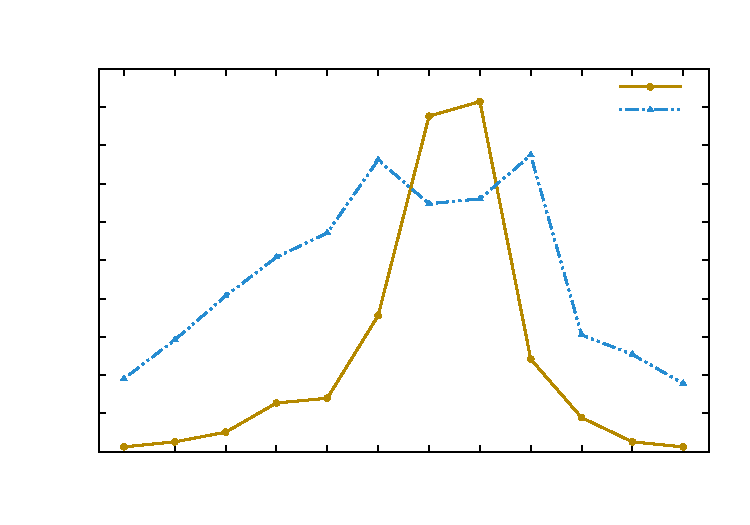
\includegraphics[width={360.00bp},height={252.00bp}]{a-inc}}%
    \gplfronttext
  \end{picture}%
\endgroup
\end{document}
